\subsection{Image  Class Reference}
\label{class_image}\index{Image@{Image}}
Class for the basic manipulation of images. 


{\tt \#include $<$image.h$>$}

Inheritance diagram for Image::\begin{figure}[H]
\begin{center}
\leavevmode
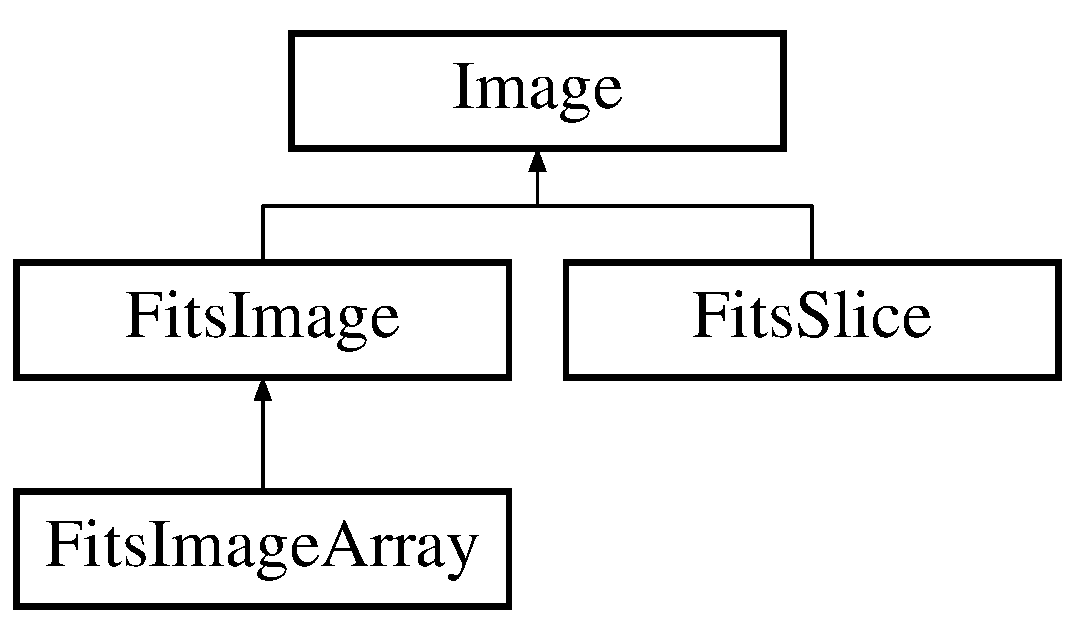
\includegraphics[height=3cm]{class_image}
\end{center}
\end{figure}
\subsubsection*{Public Methods}
\begin{CompactItemize}
\item 
\index{Image@{Image}!Image@{Image}}\index{Image@{Image}!Image@{Image}}
{\bf Image} (const int Nx, const int Ny)\label{class_image_a0}

\begin{CompactList}\small\item\em constructor reserves the needed space to store the pixels.\item\end{CompactList}\item 
\index{Image@{Image}!Image@{Image}}\index{Image@{Image}!Image@{Image}}
{\bf Image} ()\label{class_image_a1}

\begin{CompactList}\small\item\em reserves an empty image.\item\end{CompactList}\item 
\index{Image@{Image}!Image@{Image}}\index{Image@{Image}!Image@{Image}}
{\bf Image} (const Image \&)\label{class_image_a2}

\begin{CompactList}\small\item\em copy constructor.\item\end{CompactList}\item 
\index{~Image@{$\sim$Image}!Image@{Image}}\index{Image@{Image}!~Image@{$\sim$Image}}
virtual {\bf $\sim$Image} ()\label{class_image_a3}

\item 
\index{operator()@{operator()}!Image@{Image}}\index{Image@{Image}!operator()@{operator()}}
Pixel\& {\bf operator()} (const int i, const int j)\label{class_image_a4}

\begin{CompactList}\small\item\em access to the data (RW mode). The first pixel is indexed (0,0).\item\end{CompactList}\item 
\index{operator()@{operator()}!Image@{Image}}\index{Image@{Image}!operator()@{operator()}}
Pixel\& {\bf operator()} (const int i, const int j) const\label{class_image_a5}

\item 
\index{value@{value}!Image@{Image}}\index{Image@{Image}!value@{value}}
Pixel\& {\bf value} (const int i, const int j)\label{class_image_a6}

\item 
\index{MinValue@{MinValue}!Image@{Image}}\index{Image@{Image}!MinValue@{Min\-Value}}
Pixel {\bf Min\-Value} () const\label{class_image_a7}

\begin{CompactList}\small\item\em returns the minimum pixel value.\item\end{CompactList}\item 
\index{MaxValue@{MaxValue}!Image@{Image}}\index{Image@{Image}!MaxValue@{Max\-Value}}
Pixel {\bf Max\-Value} () const\label{class_image_a8}

\begin{CompactList}\small\item\em returns the maximum pixel value.\item\end{CompactList}\item 
\index{MinMaxValue@{MinMaxValue}!Image@{Image}}\index{Image@{Image}!MinMaxValue@{Min\-Max\-Value}}
void {\bf Min\-Max\-Value} (Pixel $\ast$Min, Pixel $\ast$Max) const\label{class_image_a9}

\begin{CompactList}\small\item\em returns both min and max in a single image traversal.\item\end{CompactList}\item 
\index{ClippedMeanSigmaValue@{ClippedMeanSigmaValue}!Image@{Image}}\index{Image@{Image}!ClippedMeanSigmaValue@{Clipped\-Mean\-Sigma\-Value}}
void {\bf Clipped\-Mean\-Sigma\-Value} (double \&Mean, double \&Sigma, Image $\ast$pmask=NULL) const\label{class_image_a10}

\item 
\index{MedianInFrame@{MedianInFrame}!Image@{Image}}\index{Image@{Image}!MedianInFrame@{Median\-In\-Frame}}
Pixel {\bf Median\-In\-Frame} (const {\bf Frame} \&Region, Pixel \&Sigma) const\label{class_image_a11}

\begin{CompactList}\small\item\em computes the median in a region of an image.\item\end{CompactList}\item 
\index{EnforceMinMax@{EnforceMinMax}!Image@{Image}}\index{Image@{Image}!EnforceMinMax@{Enforce\-Min\-Max}}
void {\bf Enforce\-Min\-Max} (Pixel min, Pixel max) const\label{class_image_a12}

\begin{CompactList}\small\item\em enforce the min and max value of the image.\item\end{CompactList}\item 
\index{minx@{minx}!Image@{Image}}\index{Image@{Image}!minx@{minx}}
int {\bf minx} () const\label{class_image_a13}

\item 
\index{maxx@{maxx}!Image@{Image}}\index{Image@{Image}!maxx@{maxx}}
int {\bf maxx} () const\label{class_image_a14}

\item 
\index{miny@{miny}!Image@{Image}}\index{Image@{Image}!miny@{miny}}
int {\bf miny} () const\label{class_image_a15}

\item 
\index{maxy@{maxy}!Image@{Image}}\index{Image@{Image}!maxy@{maxy}}
int {\bf maxy} () const\label{class_image_a16}

\item 
\index{MeanSigmaValue@{MeanSigmaValue}!Image@{Image}}\index{Image@{Image}!MeanSigmaValue@{Mean\-Sigma\-Value}}
void {\bf Mean\-Sigma\-Value} (Pixel $\ast$Mean, Pixel $\ast$Sigma) const\label{class_image_a17}

\begin{CompactList}\small\item\em computes the mean and sigma of an image using 5 loops over ALL image.\item\end{CompactList}\item 
\index{SkyLevel@{SkyLevel}!Image@{Image}}\index{Image@{Image}!SkyLevel@{Sky\-Level}}
void {\bf Sky\-Level} (Pixel $\ast$Mean, Pixel $\ast$Sigma) const\label{class_image_a18}

\begin{CompactList}\small\item\em computes the mean and sigma of an image using the median (from 10000 random pixels) and loop 3 times.\item\end{CompactList}\item 
\index{SkyLevel@{SkyLevel}!Image@{Image}}\index{Image@{Image}!SkyLevel@{Sky\-Level}}
void {\bf Sky\-Level} (const {\bf Frame} \&{\bf Frame}, Pixel $\ast$Mean, Pixel $\ast$Sigma) const\label{class_image_a19}

\item 
\index{Surface@{Surface}!Image@{Image}}\index{Image@{Image}!Surface@{Surface}}
void {\bf Surface} (const int Mesh\-Step, Image \&Result)\label{class_image_a20}

\begin{CompactList}\small\item\em computes a Back\-Image, subtract it, and returns the result in Result (which should have a 0 average).\item\end{CompactList}\item 
\index{dump@{dump}!Image@{Image}}\index{Image@{Image}!dump@{dump}}
void {\bf dump} () const\label{class_image_a21}

\item 
\index{Nx@{Nx}!Image@{Image}}\index{Image@{Image}!Nx@{Nx}}
int {\bf Nx} () const\label{class_image_a22}

\begin{CompactList}\small\item\em returns x size of the image.\item\end{CompactList}\item 
\index{Ny@{Ny}!Image@{Image}}\index{Image@{Image}!Ny@{Ny}}
int {\bf Ny} () const\label{class_image_a23}

\begin{CompactList}\small\item\em returns y size of the image.\item\end{CompactList}\item 
\index{operator=@{operator=}!Image@{Image}}\index{Image@{Image}!operator=@{operator=}}
Image\& {\bf operator=} (const Image \&Right)\label{class_image_a24}

\item 
\index{NPix@{NPix}!Image@{Image}}\index{Image@{Image}!NPix@{NPix}}
int {\bf NPix} () const\label{class_image_a25}

\begin{CompactList}\small\item\em returns number of pixels.\item\end{CompactList}\item 
\index{operator+@{operator+}!Image@{Image}}\index{Image@{Image}!operator+@{operator+}}
Image {\bf operator+} (const Image \&Right) const\label{class_image_a26}

\item 
\index{operator-@{operator-}!Image@{Image}}\index{Image@{Image}!operator-@{operator-}}
Image {\bf operator-} (const Image \&Right) const\label{class_image_a27}

\item 
\index{operator *@{operator $\ast$}!Image@{Image}}\index{Image@{Image}!operator *@{operator $\ast$}}
Image {\bf operator $\ast$} (const Image \&Right) const\label{class_image_a28}

\item 
\index{operator/@{operator/}!Image@{Image}}\index{Image@{Image}!operator/@{operator/}}
Image {\bf operator/} (const Image \&Right) const\label{class_image_a29}

\item 
\index{operator+=@{operator+=}!Image@{Image}}\index{Image@{Image}!operator+=@{operator+=}}
void {\bf operator+=} (const Image \&Right) const\label{class_image_a30}

\item 
\index{operator-=@{operator-=}!Image@{Image}}\index{Image@{Image}!operator-=@{operator-=}}
void {\bf operator-=} (const Image \&Right) const\label{class_image_a31}

\item 
\index{operator *=@{operator $\ast$=}!Image@{Image}}\index{Image@{Image}!operator *=@{operator $\ast$=}}
void {\bf operator $\ast$=} (const Image \&Right) const\label{class_image_a32}

\item 
\index{operator/=@{operator/=}!Image@{Image}}\index{Image@{Image}!operator/=@{operator/=}}
void {\bf operator/=} (const Image \&Right) const\label{class_image_a33}

\item 
\index{operator+@{operator+}!Image@{Image}}\index{Image@{Image}!operator+@{operator+}}
Image {\bf operator+} (const double Right) const\label{class_image_a34}

\item 
\index{operator-@{operator-}!Image@{Image}}\index{Image@{Image}!operator-@{operator-}}
Image {\bf operator-} (const double Right) const\label{class_image_a35}

\item 
\index{operator *@{operator $\ast$}!Image@{Image}}\index{Image@{Image}!operator *@{operator $\ast$}}
Image {\bf operator $\ast$} (const double Right) const\label{class_image_a36}

\item 
\index{operator/@{operator/}!Image@{Image}}\index{Image@{Image}!operator/@{operator/}}
Image {\bf operator/} (const double Right) const\label{class_image_a37}

\item 
\index{operator=@{operator=}!Image@{Image}}\index{Image@{Image}!operator=@{operator=}}
void {\bf operator=} (const double Right)\label{class_image_a38}

\item 
\index{operator+=@{operator+=}!Image@{Image}}\index{Image@{Image}!operator+=@{operator+=}}
void {\bf operator+=} (const double Right)\label{class_image_a39}

\item 
\index{operator-=@{operator-=}!Image@{Image}}\index{Image@{Image}!operator-=@{operator-=}}
void {\bf operator-=} (const double Right)\label{class_image_a40}

\item 
\index{operator *=@{operator $\ast$=}!Image@{Image}}\index{Image@{Image}!operator *=@{operator $\ast$=}}
void {\bf operator $\ast$=} (const double Right)\label{class_image_a41}

\item 
\index{operator/=@{operator/=}!Image@{Image}}\index{Image@{Image}!operator/=@{operator/=}}
void {\bf operator/=} (const double Right)\label{class_image_a42}

\item 
\index{MultiplyBySquare@{MultiplyBySquare}!Image@{Image}}\index{Image@{Image}!MultiplyBySquare@{Multiply\-By\-Square}}
void {\bf Multiply\-By\-Square} (const Image \&Right)\label{class_image_a43}

\begin{CompactList}\small\item\em multiply by the square of the image Right.\item\end{CompactList}\item 
\index{Heavyside@{Heavyside}!Image@{Image}}\index{Image@{Image}!Heavyside@{Heavyside}}
void {\bf Heavyside} ()\label{class_image_a44}

\begin{CompactList}\small\item\em pass the image trough an heaviside function that remove negative pixels.\item\end{CompactList}\item 
\index{Interpolate@{Interpolate}!Image@{Image}}\index{Image@{Image}!Interpolate@{Interpolate}}
Pixel {\bf Interpolate} (const double x, const double y, const int level=3, const bool Is\-Variance\-Map=false) const\label{class_image_a45}

\begin{CompactList}\small\item\em linear interpolation routine. I.Interpolate(0.0,0.0) returns I(0,0).\item\end{CompactList}\item 
\index{GtransfoImage@{GtransfoImage}!Image@{Image}}\index{Image@{Image}!GtransfoImage@{Gtransfo\-Image}}
Image {\bf Gtransfo\-Image} (const {\bf Gtransfo} \&g, int nx, int ny, float Default\-Val, const int interp\-Level=3, const bool Is\-Variance\-Map=false) const\label{class_image_a46}

\begin{CompactList}\small\item\em Image resampling. Can handle Variance maps.\item\end{CompactList}\item 
\index{Subimage@{Subimage}!Image@{Image}}\index{Image@{Image}!Subimage@{Subimage}}
Image {\bf Subimage} (const int x, const int y, const int width, const int height) const\label{class_image_a47}

\begin{CompactList}\small\item\em extract a subimage.\item\end{CompactList}\item 
\index{Subimage@{Subimage}!Image@{Image}}\index{Image@{Image}!Subimage@{Subimage}}
Image {\bf Subimage} (const {\bf Frame} \&frame) const\label{class_image_a48}

\begin{CompactList}\small\item\em extract a subimage.\item\end{CompactList}\item 
\index{SubimageMultiply@{SubimageMultiply}!Image@{Image}}\index{Image@{Image}!SubimageMultiply@{Subimage\-Multiply}}
void {\bf Subimage\-Multiply} (const int x, const int y, const int width, const int height, double factor)\label{class_image_a49}

\begin{CompactList}\small\item\em multiply a subimage by a double.\item\end{CompactList}\item 
\index{SubimageMultiply@{SubimageMultiply}!Image@{Image}}\index{Image@{Image}!SubimageMultiply@{Subimage\-Multiply}}
void {\bf Subimage\-Multiply} (const {\bf Frame} \&frame, double factor)\label{class_image_a50}

\begin{CompactList}\small\item\em multiply a subimage by a double.\item\end{CompactList}\item 
\index{Mask@{Mask}!Image@{Image}}\index{Image@{Image}!Mask@{Mask}}
Image {\bf Mask} (const int x\_\-Beg, const int y\_\-Beg, const int x\_\-End, const int y\_\-End) const\label{class_image_a51}

\begin{CompactList}\small\item\em keep the pixels inside the mask and put the other at 0.0.\item\end{CompactList}\item 
\index{Masking@{Masking}!Image@{Image}}\index{Image@{Image}!Masking@{Masking}}
void {\bf Masking} (const {\bf Frame} \&frame, const Pixel \&Mask\-Value=1)\label{class_image_a52}

\begin{CompactList}\small\item\em put the pixels outside mask to Mask\-Value.\item\end{CompactList}\item 
\index{DiskMaskIt@{DiskMaskIt}!Image@{Image}}\index{Image@{Image}!DiskMaskIt@{Disk\-Mask\-It}}
void {\bf Disk\-Mask\-It} (const double \&xc, const double \&yc, const double \&radius)\label{class_image_a53}

\begin{CompactList}\small\item\em put the pixels outside a disk to 1.\item\end{CompactList}\item 
\index{Truncate@{Truncate}!Image@{Image}}\index{Image@{Image}!Truncate@{Truncate}}
void {\bf Truncate} (const double \&xc, const double \&yc, const double \&radius)\label{class_image_a54}

\begin{CompactList}\small\item\em put the pixels outside a disk to 0.\item\end{CompactList}\item 
\index{Masking@{Masking}!Image@{Image}}\index{Image@{Image}!Masking@{Masking}}
void {\bf Masking} (const int x\_\-Beg, const int y\_\-Beg, const int x\_\-End, const int y\_\-End, const Pixel \&Mask\-Value=1)\label{class_image_a55}

\item 
\index{Simplify@{Simplify}!Image@{Image}}\index{Image@{Image}!Simplify@{Simplify}}
void {\bf Simplify} (double threshold, int above\_\-val=1, int under\_\-val=0)\label{class_image_a56}

\begin{CompactList}\small\item\em put pixels above threshold to 1 and to 0 otherwise.\item\end{CompactList}\item 
\index{RemoveLonePix@{RemoveLonePix}!Image@{Image}}\index{Image@{Image}!RemoveLonePix@{Remove\-Lone\-Pix}}
void {\bf Remove\-Lone\-Pix} (Image \&result, int d=1)\label{class_image_a57}

\begin{CompactList}\small\item\em remove lone bad pixels ie with no bad pixels in a square of 2d+1 x 2d+1.\item\end{CompactList}\item 
\index{SumPixels@{SumPixels}!Image@{Image}}\index{Image@{Image}!SumPixels@{Sum\-Pixels}}
double {\bf Sum\-Pixels} ()\label{class_image_a58}

\begin{CompactList}\small\item\em sum pixels values.\item\end{CompactList}\item 
\index{SumSquaredPixels@{SumSquaredPixels}!Image@{Image}}\index{Image@{Image}!SumSquaredPixels@{Sum\-Squared\-Pixels}}
double {\bf Sum\-Squared\-Pixels} () const\label{class_image_a59}

\begin{CompactList}\small\item\em sum of the squared pixel values.\item\end{CompactList}\item 
\index{MedianFilter@{MedianFilter}!Image@{Image}}\index{Image@{Image}!MedianFilter@{Median\-Filter}}
void {\bf Median\-Filter} (const int Half\-Width)\label{class_image_a60}

\item 
\index{begin@{begin}!Image@{Image}}\index{Image@{Image}!begin@{begin}}
Pixel$\ast$ {\bf begin} ()\label{class_image_a61}

\begin{CompactList}\small\item\em returns the pointer to the first pixel.\item\end{CompactList}\item 
\index{begin@{begin}!Image@{Image}}\index{Image@{Image}!begin@{begin}}
Pixel$\ast$ {\bf begin} () const\label{class_image_a62}

\item 
\index{end@{end}!Image@{Image}}\index{Image@{Image}!end@{end}}
Pixel$\ast$ {\bf end} ()\label{class_image_a63}

\begin{CompactList}\small\item\em returns the pointer to the next to last pixel, as usual for containers.\item\end{CompactList}\item 
\index{end@{end}!Image@{Image}}\index{Image@{Image}!end@{end}}
Pixel$\ast$ {\bf end} () const\label{class_image_a64}

\item 
\index{SameSize@{SameSize}!Image@{Image}}\index{Image@{Image}!SameSize@{Same\-Size}}
bool {\bf Same\-Size} (const Image \&Other) const\label{class_image_a65}

\item 
int {\bf Laplacian\-Filter} (const double \&Sigma, const double \&Mean, const double \&seeing, Image \&Cosmic\-Image)
\begin{CompactList}\small\item\em Builds a cosmic map.\item\end{CompactList}\item 
\index{Cosmics@{Cosmics}!Image@{Image}}\index{Image@{Image}!Cosmics@{Cosmics}}
void {\bf Cosmics} (const double \&Sigma, const double \&Mean, const double \&seeing, Image \&Cosmic\-Image)\label{class_image_a67}

\begin{CompactList}\small\item\em returns the final cosmic map(after iterations).\item\end{CompactList}\item 
\index{ApplyFun@{ApplyFun}!Image@{Image}}\index{Image@{Image}!ApplyFun@{Apply\-Fun}}
void {\bf Apply\-Fun} (double(\&F)(double))\label{class_image_a68}

\end{CompactItemize}
\subsubsection*{Protected Methods}
\begin{CompactItemize}
\item 
\index{allocate@{allocate}!Image@{Image}}\index{Image@{Image}!allocate@{allocate}}
void {\bf allocate} (int Nx, int Ny, int Init=1)\label{class_image_b0}

\item 
\index{get_elem_ref@{get\_\-elem\_\-ref}!Image@{Image}}\index{Image@{Image}!get_elem_ref@{get\_\-elem\_\-ref}}
Pixel$\ast$ {\bf get\_\-elem\_\-ref} (int i, int j)\label{class_image_b1}

\end{CompactItemize}
\subsubsection*{Protected Attributes}
\begin{CompactItemize}
\item 
\index{data@{data}!Image@{Image}}\index{Image@{Image}!data@{data}}
Pixel$\ast$ {\bf data}\label{class_image_n0}

\item 
\index{nx@{nx}!Image@{Image}}\index{Image@{Image}!nx@{nx}}
int {\bf nx}\label{class_image_n1}

\item 
\index{ny@{ny}!Image@{Image}}\index{Image@{Image}!ny@{ny}}
int {\bf ny}\label{class_image_n2}

\end{CompactItemize}
\subsubsection*{Friends}
\begin{CompactItemize}
\item 
class {\bf Fits\-Image\-Array}
\item 
class {\bf operator+}
\item 
class {\bf operator-}
\item 
class {\bf operator $\ast$}
\item 
class {\bf operator/}
\item 
class {\bf image\_\-copy}
\end{CompactItemize}


\subsubsection{Detailed Description}
Class for the basic manipulation of images.

The internal representation uses (32 bits) float numbers, designated later as the Pixel type. 



\subsubsection{Member Function Documentation}
\index{Image@{Image}!LaplacianFilter@{LaplacianFilter}}
\index{LaplacianFilter@{LaplacianFilter}!Image@{Image}}
\paragraph{\setlength{\rightskip}{0pt plus 5cm}int Image::Laplacian\-Filter (const double \& {\em Sigma}, const double \& {\em Mean}, const double \& {\em seeing}, Image \& {\em Cosmic\-Image})}\hfill\label{class_image_a66}


Builds a cosmic map.

Cuts (based on the article -$>$ astro-ph/0108003):  -cut\_\-lap : the laplacian operator increases the noise by a factor of  \char`\"{}sqrt(1.25)\char`\"{}

-cut\_\-f : 2$\ast$sigma(med), where sigma(med) is the variance of the sky's median calculated in a box (3$\ast$3), here.  (sigma(med) = sigma(sky)$\ast$1.22/sqrt(n); n = size of the box)

-cut\_\-lf : calculated from the article. Factor 2.35 -$>$ to have the seeing in arc sec 

The documentation for this class was generated from the following files:\begin{CompactItemize}
\item 
{\bf image.h}\item 
image.cc\end{CompactItemize}
